\section{Implementation}
\begin{figure}%
\centering
\subfigure[Visiting Statistics]{%
\label{fig:stats}%
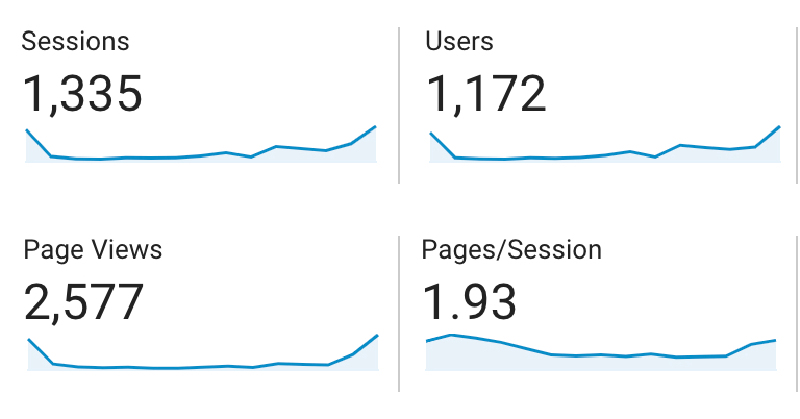
\includegraphics[width=0.23\textwidth]{figures/stats.pdf}}%
\qquad
\subfigure[Returning Users]{%
\label{fig:return}%
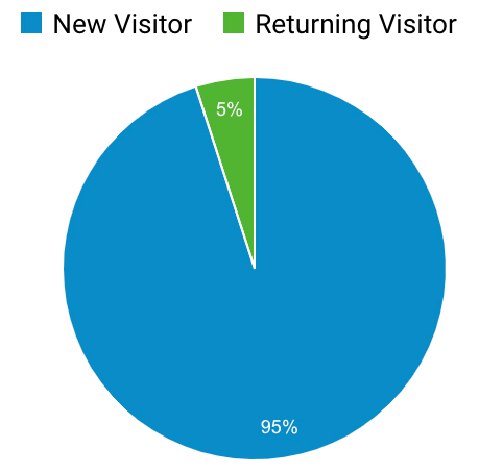
\includegraphics[width=0.17\textwidth]{figures/returning.pdf}}%
\qquad
\subfigure[Geo Map]{%
\label{fig:map}%
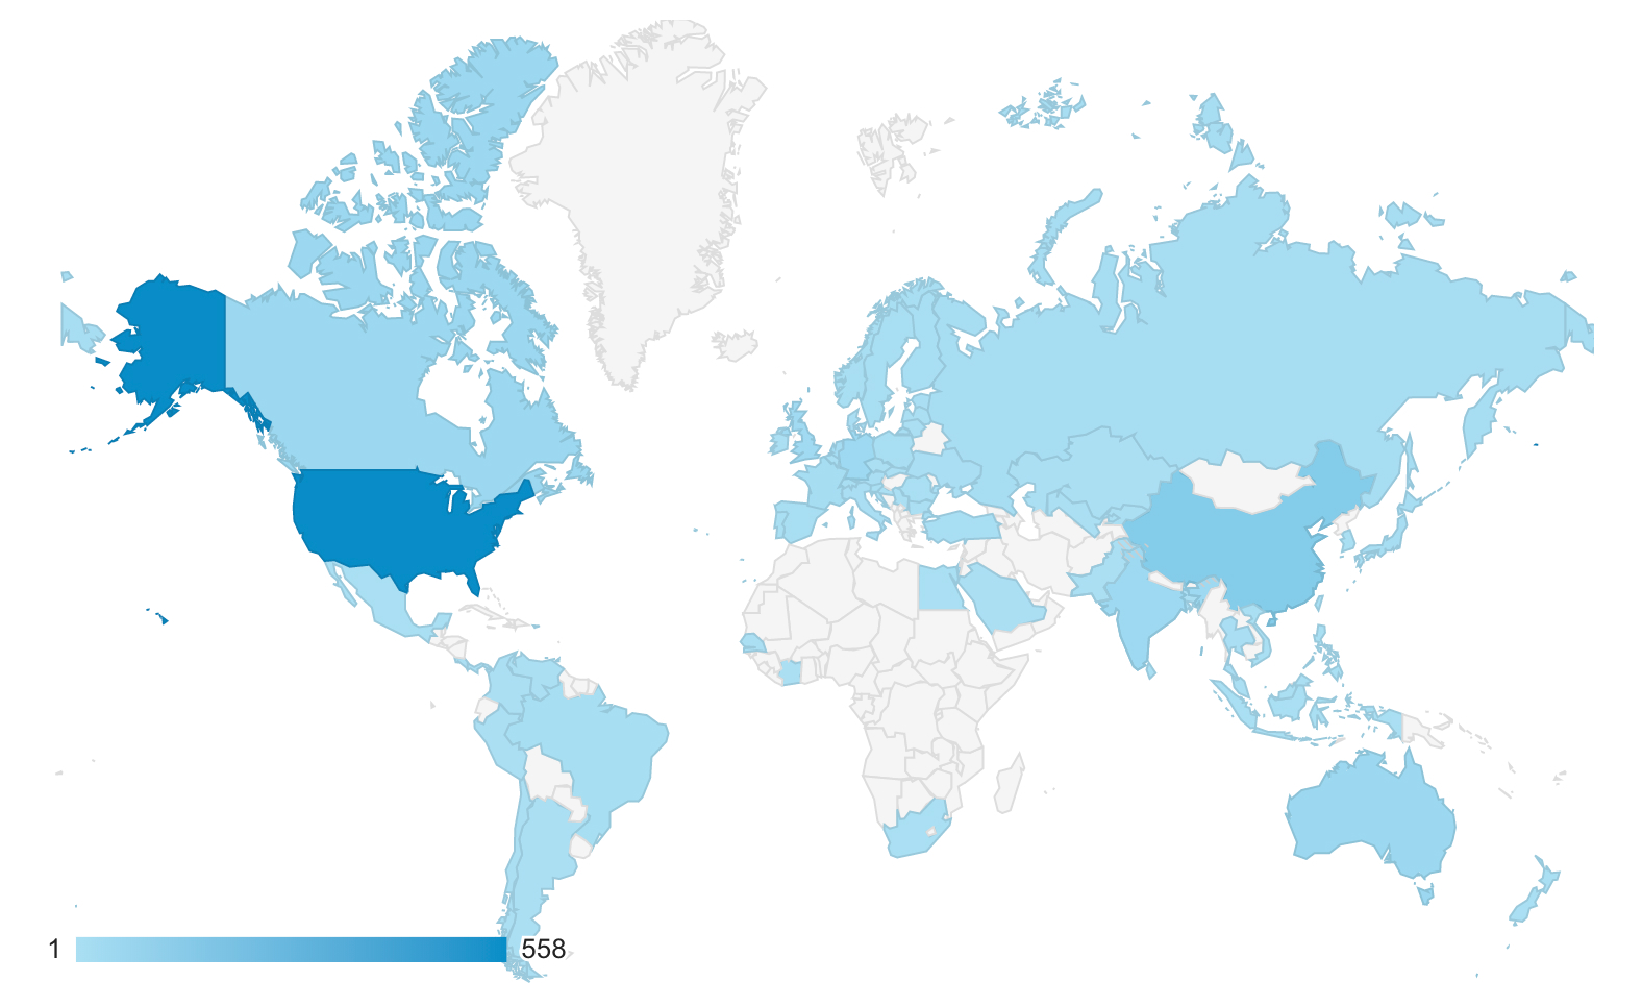
\includegraphics[width=0.4\textwidth]{figures/theworld.pdf}}%

\caption{The traffic of our website from Google Analytics\chen{This is too large, make it to a single-column figure with (a) and (c) in the first row while the map in the second row.}}
\label{fig:googleanalytics}
\end{figure}

\subsection{Dataset}
We take the latest Stack Overflow data dump (released on 4 September 2019) as the data source.
It contains 18,154,493 questions with 55,665 unique tags, and 27,765,324 answers.
With the approach in Section~\ref{sec:similarTech}, we collect in total 14,876 pairs of comparable technologies.
Among these technologies, we extract 19,118 comparative sentences for 2,410 pairs of comparable technologies.
We use these technology pairs and comparative sentences to build a knowledge base for technology comparison.

\subsection{Tool Support}
Based on the our proposed approach, we implement a practical website\footnote{\url{https://difftech.herokuapp.com/}} for developers.
With the knowledge base of comparable technologies and their comparative sentences mined from Stack Overflow, our site can return an informative and aggregated view of comparative sentences in different comparison aspects for comparable technology queries.
In addition, the tool provides the link of each comparative sentence to its corresponding Stack Overflow post so that users can easily find more detailed content. 
\wang{For example, as shown in Fig~\ref{fig:website}, given a pair of comparable technologies \textit{Gson} and \textit{Jackson}, the definition of them from TagWiki is below each technology name. 
About 69.8\% of the users support using \textit{Jackson} instead of \textit{Gson}. 
The post trend shows that \chen{although both technologies are more and more popular, there are more discussion about Jackson.}
We could also see that the method clustered all the comparative sentences into four clusters and has been clarified at the top left corner. 
For each clustered aspect, we list the comparative sentences below and attach the direct link for each comparative sentence to its original post.
User can click the link for retrieving more content.}

\subsection{Visitor Analysis}
\wang{We initially released our website on September 2018, and has updated data and layout on September 2019. We posted the news on some websites such as StackApps~\cite{??} and Reddit~\cite{??} as well for propaganda purpose. } 
\chen{You may update the following part if you have more data.}
\revise{We embedded Google Analytics into our website to monitor the site traffic. 
Fig.~\ref{fig:googleanalytics} shows that about 1,200 users from 75 different countries visited our website. 
These users viewed 2,577 different pages and in average 1.93 pages for each session. 
Note that most users come to our site with very specific target, i.e., comparing a pair of similar technologies, so, the average number of visited pages in each session is rather small.
By tracking their IP, we find that most users come from the U.S. (47.6\%), and other countries such as China (10.8\%), Australia (4\%), Canada (4\%), etc. 
Nearly 5\% of the users come back to visit our website again, indicating the usefulness and attraction of our site.
%Both the data from Google Analytics and users' comments after using our website, shows their interests and needs to our methods in comparing technologies, especially for those who are new to this area. 
}

%\wang{We find that the average page number users view per session is a bit low. This might be ascribed to the page design. For those people visiting the home page, if they can't find the desired technologies underneath, they might try to use search bar. However, it seems not clear for them to search which comparative technology pairs are available in our website. Then, for users who already is in the compare page, they might find themselves interested in certain answer ,click the question link, and end up with leaving our site to StackOverflow. }

\revise{
Among all visiting technology pairs, users compared \textit{Mysql} with \textit{Postgresql} most frequently (197 times) and other frequent technology pairs like \textit{tco vs udp}, \textit{lisp vs scheme}.
Apart from the visiting, some users also post comments under our advertisements in Reddit such as  ``\textit{Thank you ...will share the word}'', ``\textit{It was actually better than I expected, at least for the suggested comparisons. Good job!}''.
They also provide some constructive suggestion for improving our tool like \chen{``\textit{This sounds interesting. However I think it would be better if there were options to add to the technologies, pros, cons and usage.}''}, and we will further add more features in our site to make it more powerful. 
%and some suggestions on further category pros and cons for each technology. 
%In general, our website  fulfill our intention to build the site, which is to provide a platform for developers to compare similar technologies, aggregate opinions, and give suggestions. 
}





\begin{figure}
	\centering
	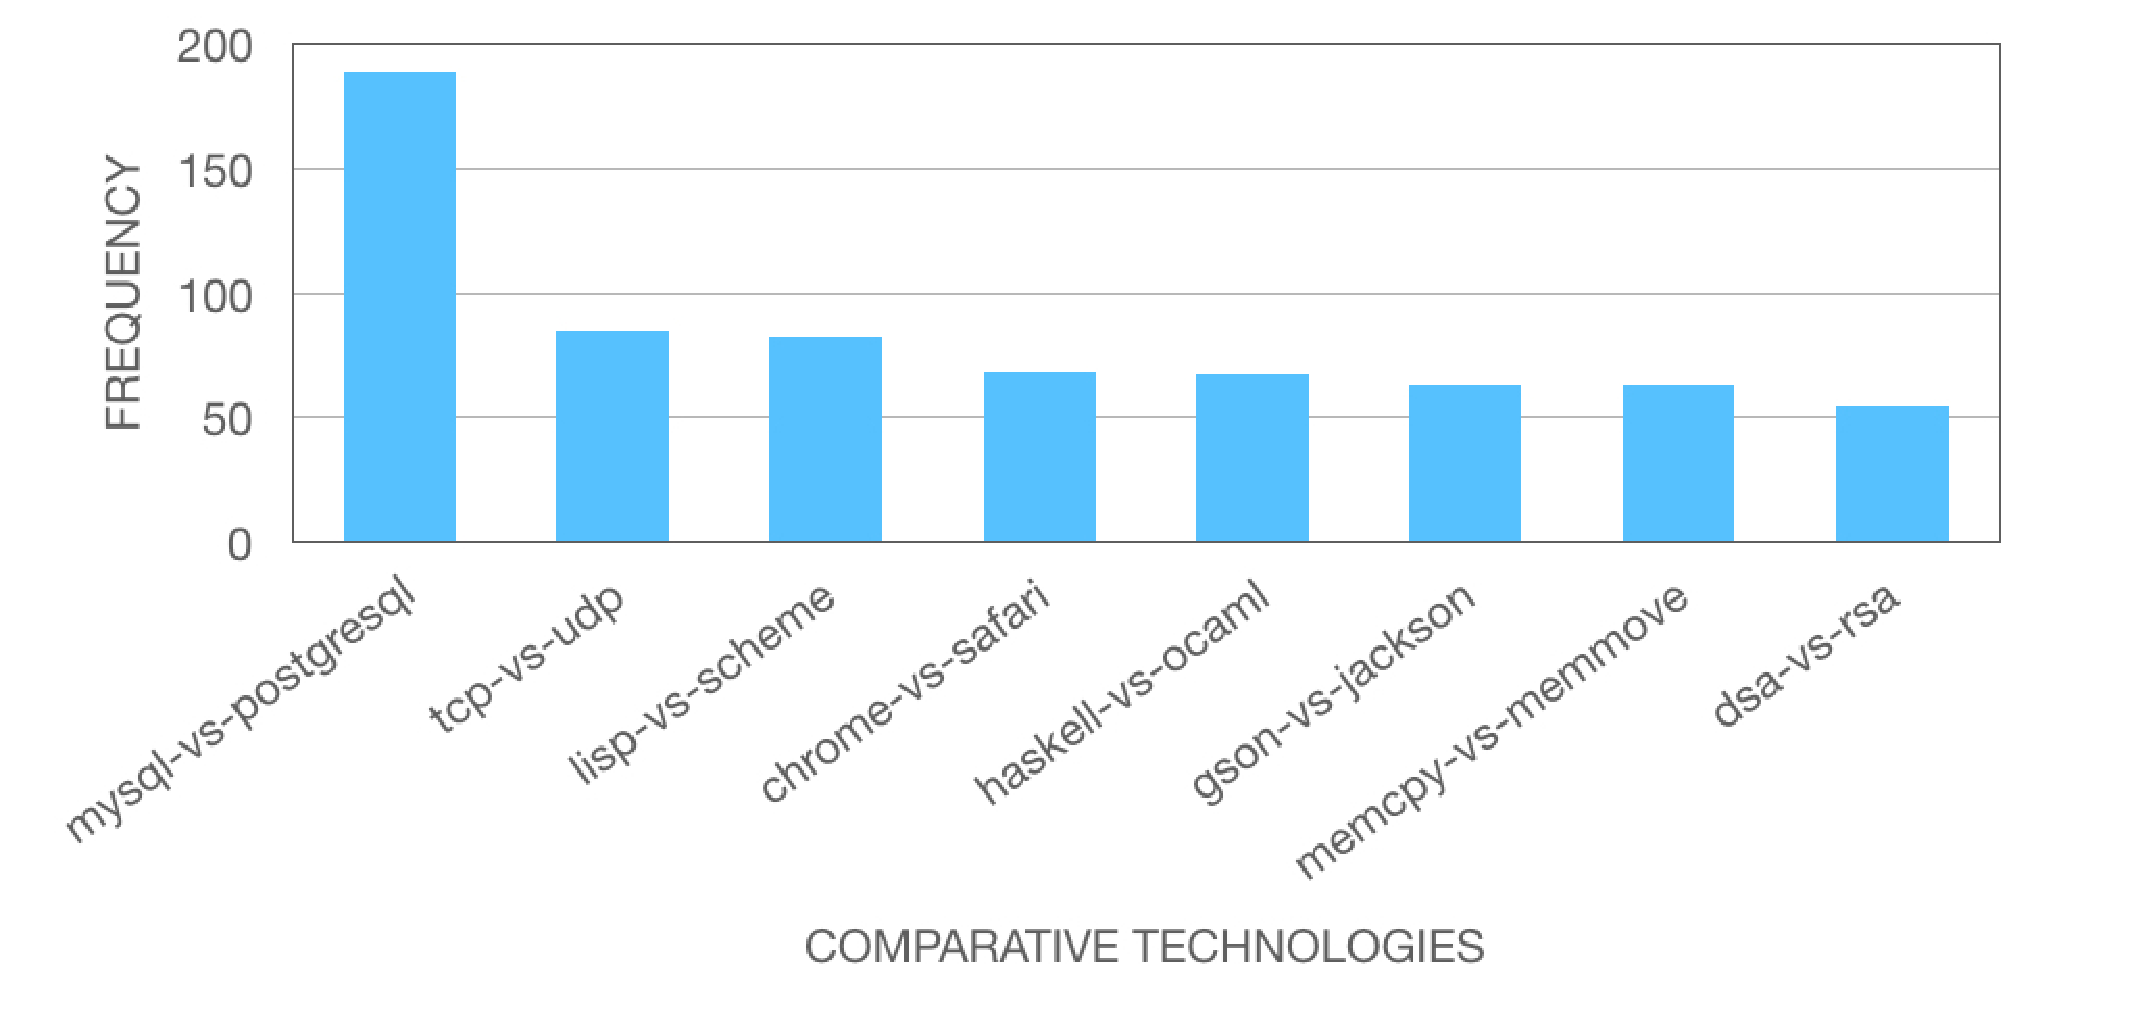
\includegraphics[width=0.49\textwidth]{figures/barChart.pdf}
	\vspace{-3mm}
	\caption{Top 8 most visited pages \chen{1)Make the labels larger 2)make it more flat for taking less vertical space.}}
	\vspace{-3mm}
	\label{fig:barChart}
\end{figure} 
